\chapter{System Architecture}
\label{ch:architecture}

This chapter presents the system architecture through various diagrams including high-level architecture, data flow diagrams, and sequence diagrams.

\section{High-Level Architecture}

Figure~\ref{fig:high-level-arch} illustrates the overall system architecture, showing the interaction between frontend, backend services, and data layer.

\begin{figure}[!htbp]
\centering
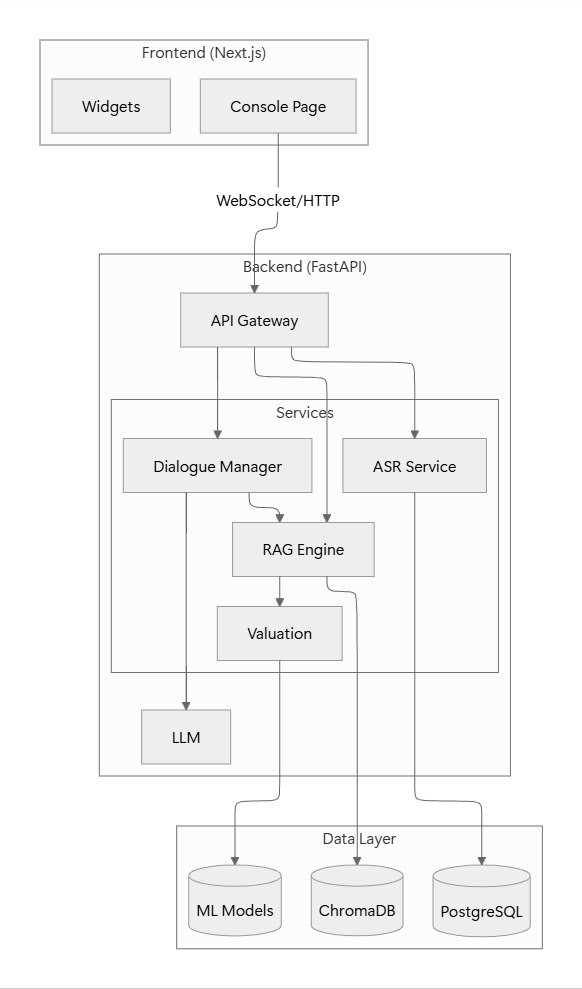
\includegraphics[width=0.95\textwidth]{ThesisFigs/High-Level_Architecture.png}
\caption{High-Level System Architecture showing Frontend, Backend Services, and Data Layer}
\label{fig:high-level-arch}
\end{figure}

The system consists of three main layers:

\begin{itemize}
    \item \textbf{Frontend (Next.js)}: Console page for agent interaction, UI widgets for displaying prices and listings, and waveform visualizer for audio feedback
    \item \textbf{Backend (FastAPI)}: API gateway routing to core services including ASR, Dialogue Manager, RAG Engine, and Valuation services
    \item \textbf{Data Layer}: ChromaDB for vector storage, PostgreSQL for structured data, and ML models for ASR and price prediction
\end{itemize}

The frontend communicates with the backend via WebSocket for real-time audio streaming and HTTP for dialogue API calls. The LLM module interfaces with either Google's Gemini API or local HuggingFace models.

\section{Data Flow Diagram - Level 0 (Context)}

Figure~\ref{fig:dfd-0} shows the context-level data flow diagram identifying external entities and their interactions with the Voice Agent System.

\begin{figure}[!htbp]
\centering
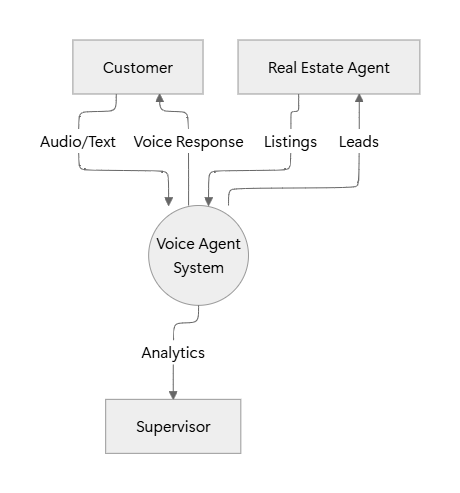
\includegraphics[width=0.7\textwidth]{ThesisFigs/Data_Flow_Diagram_Level_0.png}
\caption{Context-Level DFD showing external entities interacting with the Voice Agent System}
\label{fig:dfd-0}
\end{figure}

Three external entities interact with the system:

\begin{itemize}
    \item \textbf{Customer}: Sends audio/text input and receives voice responses with property information
    \item \textbf{Real Estate Agent}: Provides property listings and receives qualified leads with call summaries
    \item \textbf{Supervisor}: Receives analytics and KPIs for performance monitoring
\end{itemize}

\section{Data Flow Diagram - Level 1}

Figure~\ref{fig:dfd-1} decomposes the system into its major processing components and data stores.

\begin{figure}[!htbp]
\centering
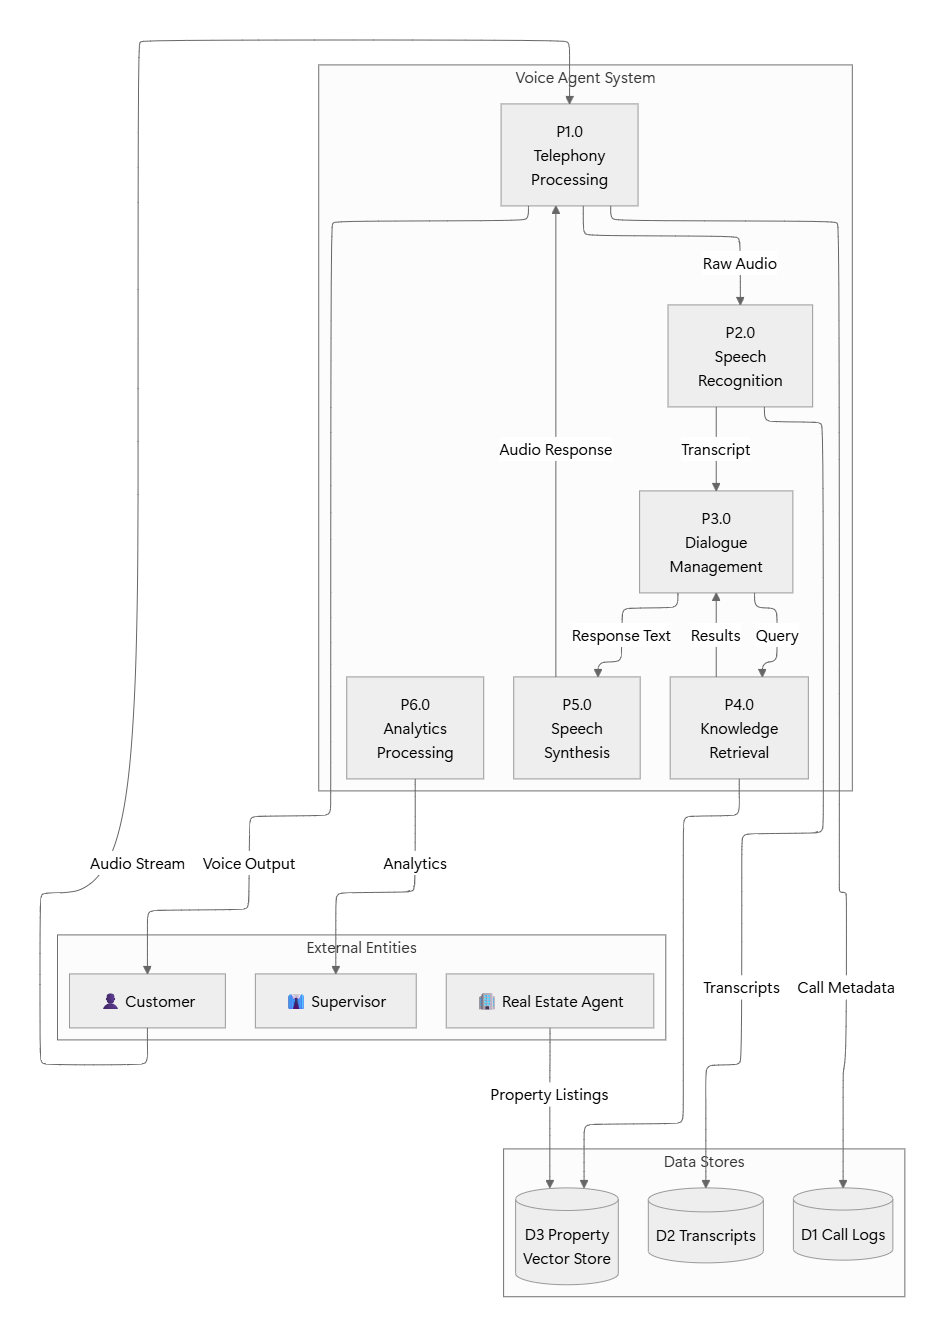
\includegraphics[width=0.95\textwidth]{ThesisFigs/Data_Flow_Diagram_Level_1.png}
\caption{Level 1 DFD showing major system processes and data flows}
\label{fig:dfd-1}
\end{figure}

The Level 1 DFD reveals six major processes:

\begin{enumerate}
    \item \textbf{P1.0 Telephony Processing}: Handles audio stream capture and playback
    \item \textbf{P2.0 Speech Recognition}: Converts audio to text transcripts using Whisper ASR
    \item \textbf{P3.0 Dialogue Management}: Processes transcripts, manages context, and generates responses
    \item \textbf{P4.0 Knowledge Retrieval}: Searches the property vector store for relevant listings
    \item \textbf{P5.0 Speech Synthesis}: Converts response text to audio (Iteration 3)
    \item \textbf{P6.0 Analytics Processing}: Generates reports and KPIs for supervisors
\end{enumerate}

The data stores include:
\begin{itemize}
    \item \textbf{D1 Call Logs}: Stores call metadata and recordings
    \item \textbf{D2 Transcripts}: Stores conversation transcripts
    \item \textbf{D3 Property Vector Store}: ChromaDB collection of property embeddings
\end{itemize}

\section{DFD Level 2 - Dialogue Management}

Figure~\ref{fig:dfd-2} provides a detailed view of the Dialogue Management process (P3.0), showing the sub-processes involved in generating responses.

\begin{figure}[!htbp]
\centering
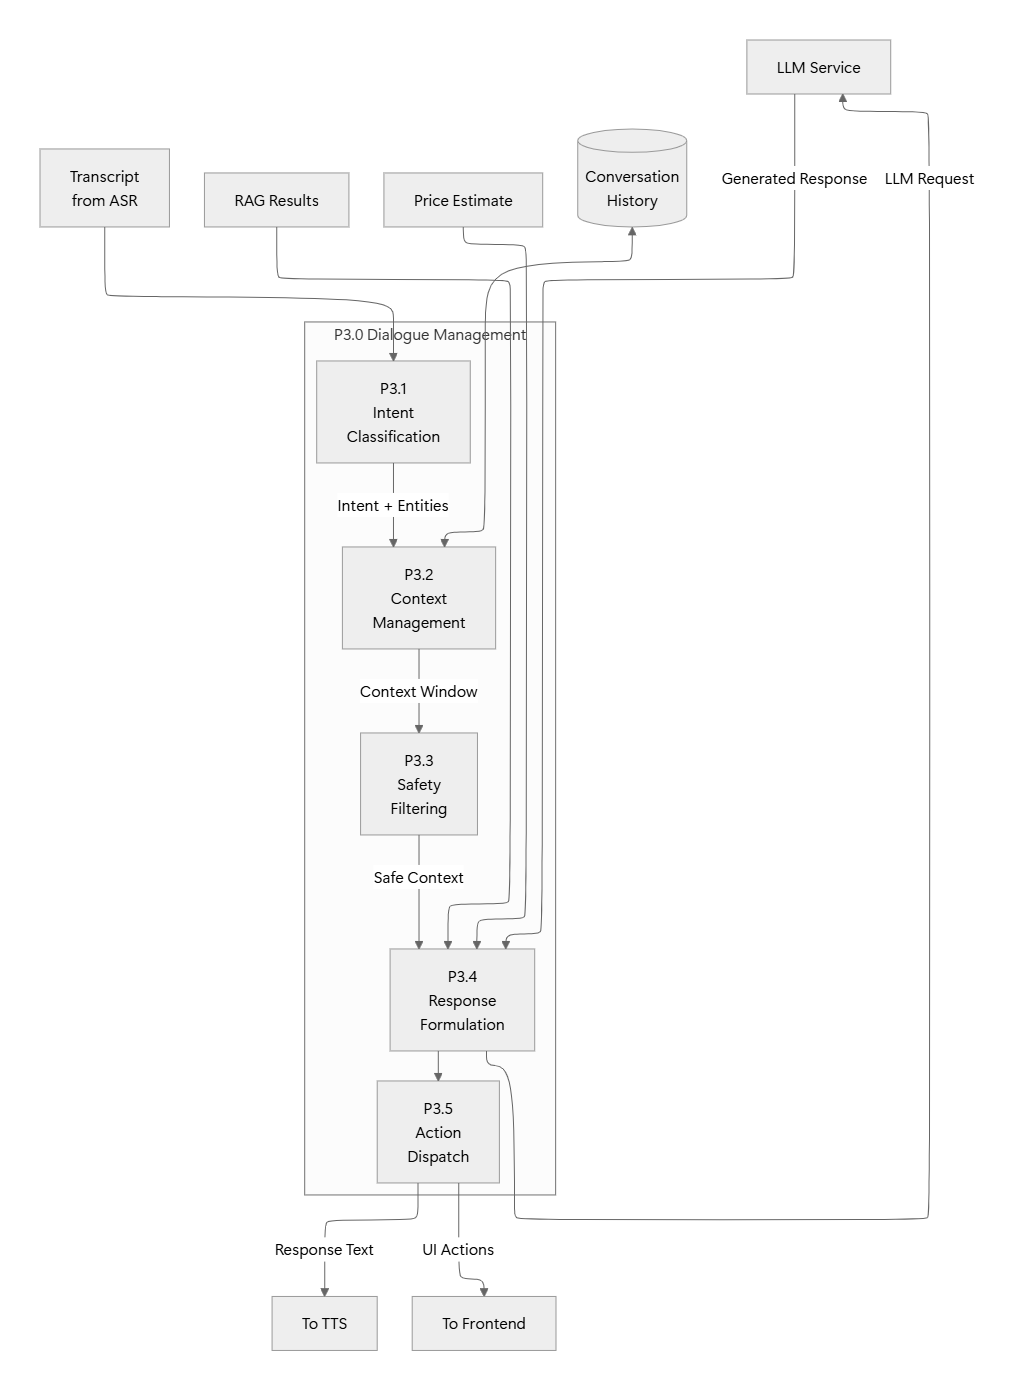
\includegraphics[width=0.95\textwidth]{ThesisFigs/Data_Flow_Diagram_Level_2_Dialogue_Management.png}
\caption{Level 2 DFD detailing the Dialogue Management process}
\label{fig:dfd-2}
\end{figure}

The dialogue management process comprises five sub-processes:

\begin{enumerate}
    \item \textbf{P3.1 Intent Classification}: Determines user intent (price query, property search, booking)
    \item \textbf{P3.2 Context Management}: Maintains conversation history and session state
    \item \textbf{P3.3 Safety Filtering}: Ensures responses are appropriate and accurate
    \item \textbf{P3.4 Response Formulation}: Constructs prompts and generates LLM responses
    \item \textbf{P3.5 Action Dispatch}: Routes responses and triggers appropriate UI widgets
\end{enumerate}

The process integrates RAG results and price estimates into the context before sending to the LLM for response generation.

\section{Sequence Diagram - Dialogue Turn}

Figure~\ref{fig:sequence} illustrates a complete dialogue turn from user speech to agent response, showing the timing and interaction between components.

\begin{figure}[!htbp]
\centering
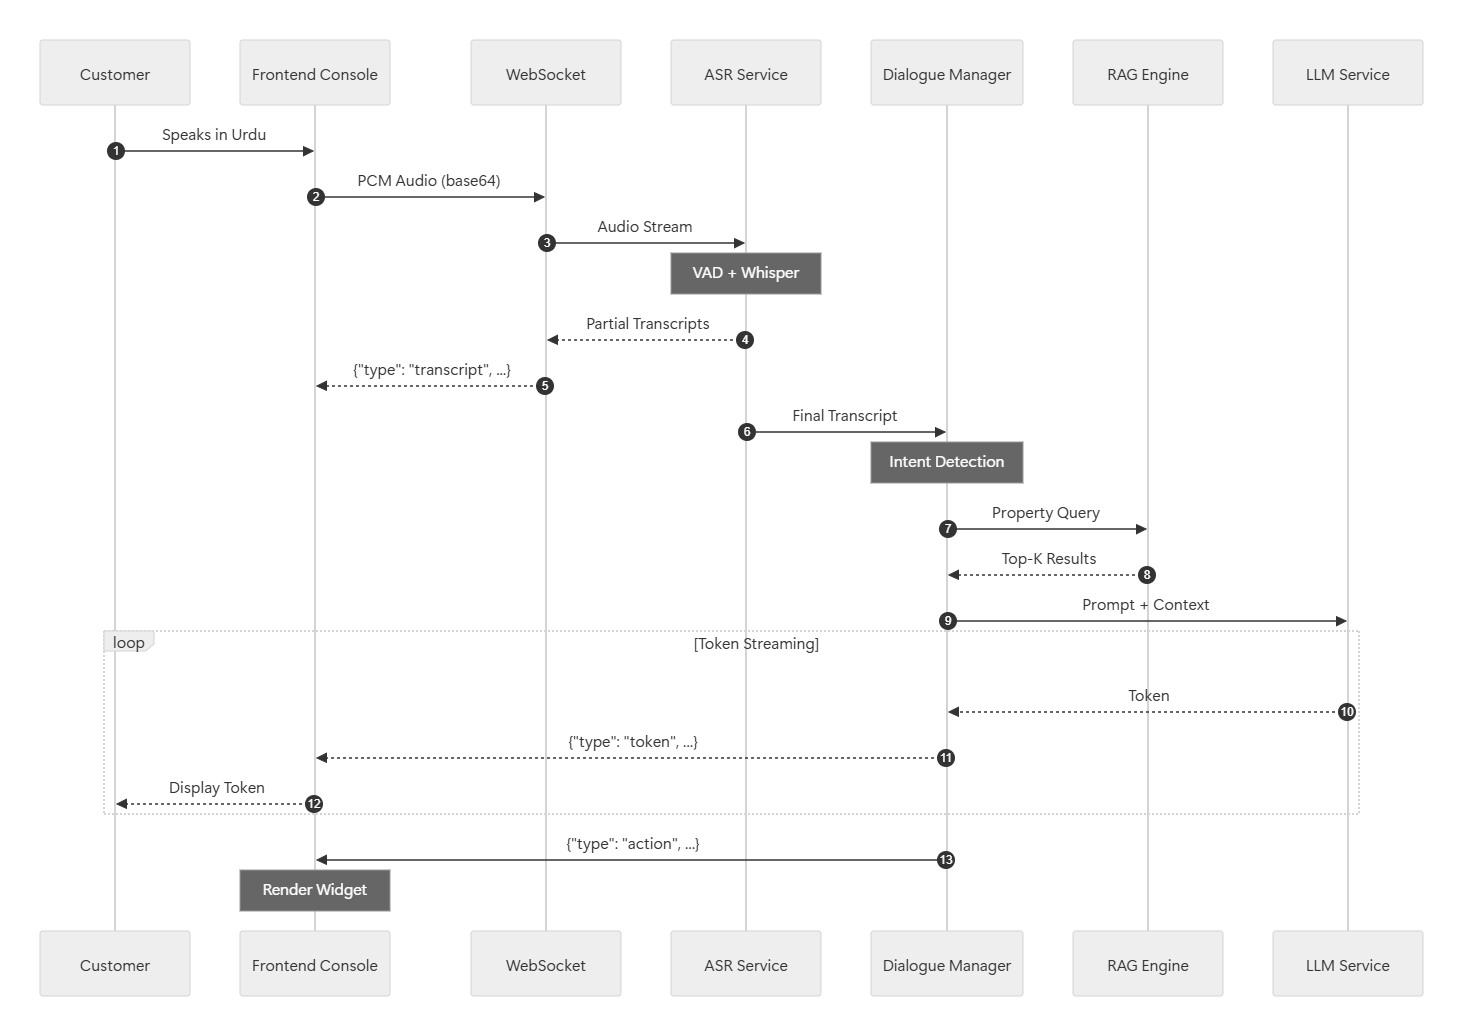
\includegraphics[width=0.95\textwidth]{ThesisFigs/Sequence Diagram - Dialogue Turn}
\caption{Sequence diagram showing a complete dialogue turn with streaming response}
\label{fig:sequence}
\end{figure}

The sequence of events in a typical dialogue turn:

\begin{enumerate}
    \item Customer speaks in Urdu
    \item Frontend captures PCM audio and sends via WebSocket
    \item ASR Service applies VAD and Whisper transcription
    \item Partial transcripts are streamed back to frontend
    \item Final transcript is sent to Dialogue Manager
    \item Dialogue Manager detects intent and queries RAG Engine
    \item RAG Engine returns top-K property results
    \item Dialogue Manager constructs prompt with context and sends to LLM
    \item LLM streams tokens back through the Dialogue Manager
    \item Frontend displays tokens progressively and renders action widgets
\end{enumerate}

\section{State Diagram - Dialogue States}

The dialogue system maintains conversation state to track progress through the lead qualification process. The main states are:

\begin{itemize}
    \item \textbf{Greeting}: Initial state when session starts
    \item \textbf{QualifyingLead}: Main conversation state for understanding customer needs
    \item \textbf{ProvidingInfo}: Sharing property details based on search results
    \item \textbf{GivingQuote}: Presenting price estimates
    \item \textbf{Scheduling}: Booking property visits or appointments
    \item \textbf{Confirmation}: Confirming appointment details
    \item \textbf{Closing}: End of conversation
\end{itemize}

State transitions occur based on detected user intents and the natural flow of conversation. The system can move between ProvidingInfo, GivingQuote, and Scheduling states multiple times before reaching Closing.
